\documentclass[tikz,border=6pt]{standalone}
\usepackage[T1]{fontenc}
\usepackage{times}
\usepackage{amsmath,amssymb,bm}
\DeclareMathOperator*{\argmin}{arg\,min}
\usetikzlibrary{arrows.meta, positioning, fit, backgrounds, calc, decorations.pathreplacing}

% Colors
\definecolor{nncolor}{HTML}{FAD7A0}
\definecolor{nnborder}{HTML}{E67E22}
\definecolor{mpccolor}{HTML}{A9DFBF}
\definecolor{mpcborder}{HTML}{27AE60}
\definecolor{criticcolor}{HTML}{D7BDE2}
\definecolor{criticborder}{HTML}{8E44AD}
\definecolor{actorbg}{HTML}{FEF9E7}
\definecolor{actorborder}{HTML}{D4AC0D}
\definecolor{neuroncolor}{HTML}{5DADE2}

\begin{document}
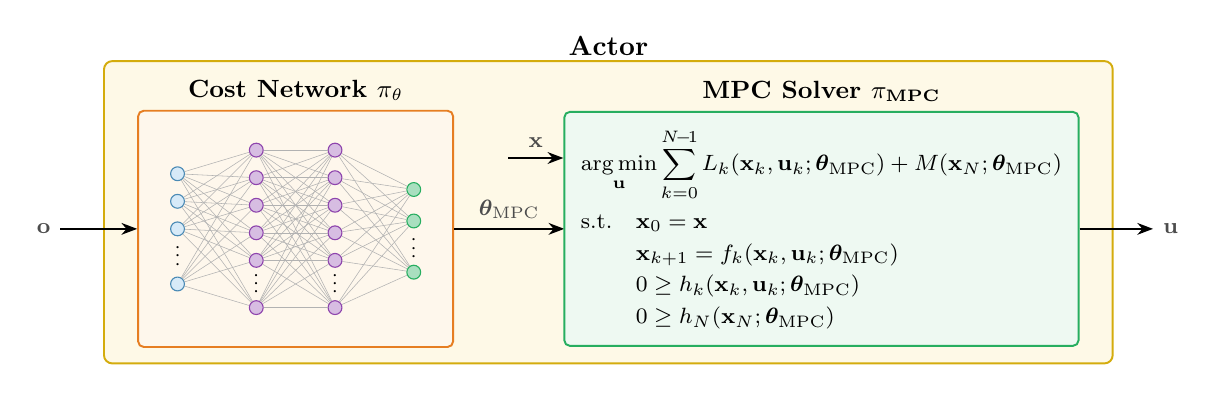
\begin{tikzpicture}[
    >=Stealth,
    block/.style={draw, rounded corners=2pt, minimum height=0.85cm,
        minimum width=1.7cm, align=center, font=\small, line width=0.7pt},
    nn/.style={block, fill=nncolor, draw=nnborder},
    mpc/.style={block, fill=mpccolor, draw=mpcborder},
    actorbox/.style={draw=actorborder, rounded corners=3pt,
        fill=actorbg, inner sep=6pt, line width=0.7pt},
    dl/.style={font=\footnotesize, text=black!70},
    arr/.style={->, line width=0.6pt},
    neuron/.style={circle, draw=neuroncolor!80!black, fill=neuroncolor!25,
        minimum size=5pt, inner sep=0pt, line width=0.4pt},
    mpcdetail/.style={draw=mpcborder, rounded corners=2pt,
        fill=mpccolor!20, inner sep=6pt, line width=0.7pt,
        align=left, font=\footnotesize},
    nndetail/.style={draw=nnborder, rounded corners=2pt,
        fill=nncolor!20, inner sep=6pt, line width=0.7pt},
]

% --- Neural Network Neurons ---
\node[nndetail, minimum width=4.0cm, minimum height=3.0cm]
    (nnbox) at (-4.0, -7.5) {};
\node[font=\small\bfseries, anchor=south] at (nnbox.north)
    {Cost Network $\pi_\theta$};

\begin{scope}
% Input layer (3 top + vdots + 1 bottom) — centered
\foreach \i/\y in {1/0.7, 2/0.35, 3/0.0} {
    \node[neuron] (in\i) at (-5.5, -7.5+\y) {};
}
\node[font=\scriptsize, text=black, inner sep=0pt, anchor=north, align=center] at (-5.5, -7.5-0.18) {$\cdot$\\[-5pt]$\cdot$\\[-5pt]$\cdot$};
\foreach \i/\y in {4/-0.7} {
    \node[neuron] (in\i) at (-5.5, -7.5+\y) {};
}
% Hidden layer 1 (5 top + vdots + 1 bottom) — centered
\foreach \i/\y in {1/1.0, 2/0.65, 3/0.3, 4/-0.05, 5/-0.4} {
    \node[neuron, draw=criticborder, fill=criticcolor] (h1\i) at (-4.5, -7.5+\y) {};
}
\node[font=\scriptsize, text=black, inner sep=0pt, anchor=north, align=center] at (-4.5, -7.5-0.53) {$\cdot$\\[-5pt]$\cdot$\\[-5pt]$\cdot$};
\foreach \i/\y in {6/-1.0} {
    \node[neuron, draw=criticborder, fill=criticcolor] (h1\i) at (-4.5, -7.5+\y) {};
}
% Hidden layer 2 (5 top + vdots + 1 bottom) — centered
\foreach \i/\y in {1/1.0, 2/0.65, 3/0.3, 4/-0.05, 5/-0.4} {
    \node[neuron, draw=criticborder, fill=criticcolor] (h2\i) at (-3.5, -7.5+\y) {};
}
\node[font=\scriptsize, text=black, inner sep=0pt, anchor=north, align=center] at (-3.5, -7.5-0.53) {$\cdot$\\[-5pt]$\cdot$\\[-5pt]$\cdot$};
\foreach \i/\y in {6/-1.0} {
    \node[neuron, draw=criticborder, fill=criticcolor] (h2\i) at (-3.5, -7.5+\y) {};
}
% Output layer (2 top + vdots + 1 bottom) — centered
\foreach \i/\y in {1/0.5, 2/0.1} {
    \node[neuron, draw=mpcborder, fill=mpccolor] (out\i) at (-2.5, -7.5+\y) {};
}
\node[font=\scriptsize, text=black, inner sep=0pt, anchor=north, align=center] at (-2.5, -7.5-0.08) {$\cdot$\\[-5pt]$\cdot$\\[-5pt]$\cdot$};
\foreach \i/\y in {3/-0.55} {
    \node[neuron, draw=mpcborder, fill=mpccolor] (out\i) at (-2.5, -7.5+\y) {};
}
% Connections: input -> hidden1
\foreach \i in {1,2,3,4} {
    \foreach \j in {1,2,3,4,5,6} {
        \draw[line width=0.2pt, black!30] (in\i) -- (h1\j);
    }
}
% Connections: hidden1 -> hidden2
\foreach \i in {1,2,3,4,5,6} {
    \foreach \j in {1,2,3,4,5,6} {
        \draw[line width=0.2pt, black!30] (h1\i) -- (h2\j);
    }
}
% Connections: hidden2 -> output
\foreach \i in {1,2,3,4,5,6} {
    \foreach \j in {1,2,3} {
        \draw[line width=0.2pt, black!30] (h2\i) -- (out\j);
    }
}
% Input label (outside nnbox, with arrow into nnbox)
\node[dl] (oilabel) at (-7.2, -7.5) {$\mathbf{o}$};
\draw[arr] (oilabel.east) -- (nnbox.west);
\end{scope}

% Arrow from NN box to MPC box
\draw[arr] (nnbox.east) -- ++(1.4, 0)
    node[dl, above, midway] {$\bm{\theta}_{\text{MPC}}$};

% --- MPC Equation Block ---
\node[mpcdetail, anchor=west] (mpcbox) at (-0.6, -7.5) {%
$\displaystyle \argmin_{\mathbf{u}}
\sum_{k=0}^{N\!-\!1} L_k(\mathbf{x}_k, \mathbf{u}_k; \bm{\theta}_{\text{MPC}})
+ M(\mathbf{x}_N;\bm{\theta}_{\text{MPC}})$\\[4pt]
$\text{s.t.}\quad \mathbf{x}_0 = \mathbf{x}$\\[2pt]
$\phantom{\text{s.t.}}\quad \mathbf{x}_{k+1}
= f_k(\mathbf{x}_k, \mathbf{u}_k;\bm{\theta}_{\text{MPC}})$\\[2pt]
$\phantom{\text{s.t.}}\quad 0 \geq
h_k(\mathbf{x}_k, \mathbf{u}_k;\bm{\theta}_{\text{MPC}})$\\[2pt]
$\phantom{\text{s.t.}}\quad 0 \geq
h_N(\mathbf{x}_N;\bm{\theta}_{\text{MPC}})$%
};
\node[font=\small\bfseries, anchor=south] at (mpcbox.north)
    {MPC Solver $\pi_{\text{MPC}}$};

% x input to MPC (arrow into left side of block)
\draw[arr] ([xshift=-0.7cm, yshift=0.9cm]mpcbox.west)
    -- node[dl, above] {$\mathbf{x}$} ([yshift=0.9cm]mpcbox.west);

% Actor box inside detail
\coordinate (detact-top-pad) at ([yshift=18pt]mpcbox.north);
\coordinate (detact-bot-pad) at ([yshift=-6pt]mpcbox.south);
\begin{scope}[on background layer]
\node[actorbox, fit=(nnbox)(mpcbox)(detact-top-pad)(detact-bot-pad), inner xsep=12pt, inner ysep=0pt,
    label={[font=\normalsize\bfseries, yshift=-2pt]above:Actor}] (detact) {};
\end{scope}

% Action output from MPC (right, past actor box)
\draw[arr] (mpcbox.east) -- (detact.east |- mpcbox.east) -- ++(0.5, 0)
    node[dl, right] {$\mathbf{u}$};

\end{tikzpicture}
\end{document}
